% Options for packages loaded elsewhere
\PassOptionsToPackage{unicode}{hyperref}
\PassOptionsToPackage{hyphens}{url}
\PassOptionsToPackage{dvipsnames,svgnames,x11names}{xcolor}
\documentclass[
]{ltjsarticle}
\usepackage{xcolor}
\usepackage[margin=20mm]{geometry}
\usepackage{amsmath,amssymb}
\setcounter{secnumdepth}{-\maxdimen} % remove section numbering
\usepackage{iftex}
\ifPDFTeX
  \usepackage[T1]{fontenc}
  \usepackage[utf8]{inputenc}
  \usepackage{textcomp} % provide euro and other symbols
\else % if luatex or xetex
  \usepackage{unicode-math} % this also loads fontspec
  \defaultfontfeatures{Scale=MatchLowercase}
  \defaultfontfeatures[\rmfamily]{Ligatures=TeX,Scale=1}
\fi
\usepackage{lmodern}
\ifPDFTeX\else
  % xetex/luatex font selection
\fi
% Use upquote if available, for straight quotes in verbatim environments
\IfFileExists{upquote.sty}{\usepackage{upquote}}{}
\IfFileExists{microtype.sty}{% use microtype if available
  \usepackage[]{microtype}
  \UseMicrotypeSet[protrusion]{basicmath} % disable protrusion for tt fonts
}{}
\makeatletter
\@ifundefined{KOMAClassName}{% if non-KOMA class
  \IfFileExists{parskip.sty}{%
    \usepackage{parskip}
  }{% else
    \setlength{\parindent}{0pt}
    \setlength{\parskip}{6pt plus 2pt minus 1pt}}
}{% if KOMA class
  \KOMAoptions{parskip=half}}
\makeatother
\usepackage{longtable,booktabs,array}
\newcounter{none} % for unnumbered tables
\usepackage{calc} % for calculating minipage widths
% Correct order of tables after \paragraph or \subparagraph
\usepackage{etoolbox}
\makeatletter
\patchcmd\longtable{\par}{\if@noskipsec\mbox{}\fi\par}{}{}
\makeatother
% Allow footnotes in longtable head/foot
\IfFileExists{footnotehyper.sty}{\usepackage{footnotehyper}}{\usepackage{footnote}}
\makesavenoteenv{longtable}
\usepackage{graphicx}
\makeatletter
\newsavebox\pandoc@box
\newcommand*\pandocbounded[1]{% scales image to fit in text height/width
  \sbox\pandoc@box{#1}%
  \Gscale@div\@tempa{\textheight}{\dimexpr\ht\pandoc@box+\dp\pandoc@box\relax}%
  \Gscale@div\@tempb{\linewidth}{\wd\pandoc@box}%
  \ifdim\@tempb\p@<\@tempa\p@\let\@tempa\@tempb\fi% select the smaller of both
  \ifdim\@tempa\p@<\p@\scalebox{\@tempa}{\usebox\pandoc@box}%
  \else\usebox{\pandoc@box}%
  \fi%
}
% Set default figure placement to htbp
\def\fps@figure{htbp}
\makeatother
\setlength{\emergencystretch}{3em} % prevent overfull lines
\providecommand{\tightlist}{%
  \setlength{\itemsep}{0pt}\setlength{\parskip}{0pt}}
\usepackage{float}
\floatplacement{figure}{H}
\usepackage{bookmark}
\IfFileExists{xurl.sty}{\usepackage{xurl}}{} % add URL line breaks if available
\urlstyle{same}
\hypersetup{
  colorlinks=true,
  linkcolor={Maroon},
  filecolor={Maroon},
  citecolor={Blue},
  urlcolor={Blue},
  pdfcreator={LaTeX via pandoc}}

\author{}
\date{}

\begin{document}

\section{論文0:正曲率定曲率空間における測地的単位セルの歪み ---
一辺・角・面積・体積の厳密評価}\label{ux8ad6ux65870ux6b63ux66f2ux7387ux5b9aux66f2ux7387ux7a7aux9593ux306bux304aux3051ux308bux6e2cux5730ux7684ux5358ux4f4dux30bbux30ebux306eux6b6aux307f-ux4e00ux8fbaux89d2ux9762ux7a4dux4f53ux7a4dux306eux53b3ux5bc6ux8a55ux4fa1}

\textbf{著者}: 木原範昭(Noriaki Kihara) \textbf{所属}: WF System Co.,
Ltd.~/ ORCID: 0009-0004-6753-4020 \textbf{DOI}: Version
10.5281/zenodo.20684135（本版）/ Concept
10.5281/zenodo.20680269（外部参照用・最新版へ自動転送） \textbf{Zenodo}:
https://zenodo.org/records/20684135 \textbf{版}: v1.4(v1.3 に §4.6
の先行研究段落{[}スペクトル次元・Böröczky・Schläfli
との差別化{]}と外部参考文献を追加、§1 に存在閾値の Schläfli
的位置づけを一文、付録A の数式組版を正式 LaTeX に修正。v1.3 は v1.2
に実計算図5点を挿入。図は全て厳密計算、模式図なし。二者検算プロトコル)
\textbf{位置づけ}:本稿は基礎篇・\textbf{論文0}であり、補正対象は論文1〜2
の平坦数え上げ(§5)。論文一覧.md・総説参考文献への論文0 行の追加と論文1
との相互リンクは出版管理として別途行う(本稿確定後)。
\textbf{本稿の七観点}:
一辺(1)・頂点角(2)・面積(3)・体積(4)・曲率の逆算(4.5)・次元の曖昧さと共役量(4.6)・次元創発と
d=4 ロック(4.7)。全数値は同梱スクリプトで再現可能、検算6項目すべて合格。
\textbf{シリーズ}: 波長空間と周波数空間の双対幾何(基礎篇・論文0)
\textbf{検算スクリプト}: \texttt{paper0\_geodesic\_cell\_distortion.py}

\begin{center}\rule{0.5\linewidth}{0.5pt}\end{center}

\subsection{0. 本稿の位置づけ ---
歪問題の明確な定義}\label{ux672cux7a3fux306eux4f4dux7f6eux3065ux3051-ux6b6aux554fux984cux306eux660eux78baux306aux5b9aux7fa9}

本シリーズはこれまで、基礎写像として球面投影
σ\_R(x)=(R/‖x‖)x(球面投影編「中心投影シリーズ:radial projection σ\_R
の基礎写像」Concept DOI 10.5281/zenodo.20462569 ---
本シリーズ(論文1〜16)とは別系列の外部参照。論文一覧.md
には載らないシリーズ外文献として扱う)と、その接超平面 Π\_R
への制限である中心投影 Φ\_R(中心投影編)を用いてきた。σ\_R
は方向・角度を保つ一方で距離を保たず、その歪みは「単一点では現れず、点と点の関係(相対配置・間隔)としてのみ顕在化する」(球面投影編
観察2.7)。\textbf{しかし、この歪みを一辺・頂点角・面積・体積として定量的に書き下すことは、これまでどの論文でも明確には定式化されてこなかった}------球面投影編
§4.3
は誘導計量・曲率としての定式化を別論文へ明示的に延期し、論文1以降の数え上げは拘束
Σν\(^{2}\)=\(\mathcal{N}\)\(^{2}\) が定義する曲面 S\^{}d(R) の内在曲率を
4 自由度の数え上げに取り込まないまま平坦ノルムで進めていた。

\textbf{本稿の目的は、この延期されてきた「歪問題」------曲率半径 R
の正曲率定曲率空間に置かれた単位セルの幾何学的歪み------を、純粋な微分幾何の基礎計算として明確に定義することである。}
ただし重要な精密化を先に述べる:論文1〜2
の平坦扱いは\textbf{不足ではなく、1次元波の内容に対しては曲率厳密}である(§2:d=1
は内在的平坦で歪みゼロ;§4.8)。歪み(§3〜4、d≥2)が現れるのは複数軸を結合した真の測地胞体に限られ、そここそシリーズが振幅なし論理波(論文9
§2.3「曲率整合」)で扱う対象である。本稿は「平坦扱いが厳密に成立する境界の画定」として読むのが正確で、§5
の補正は多次元測地胞体への読み替えに対する平均場見積もりに限られる。
確率も測度も振幅も登場しない。問うのはただ一つ:

\begin{quote}
正準化(離散単位=1、バラツキ ±½、曲率半径
R)の下で、平坦な単位セルを曲率半径 R
の正曲率定曲率空間に\textbf{測地線長を保って}置いたとき、一辺・頂点角・面積・体積はどう変わるか。
\end{quote}

基礎写像を従来「中心投影」「球面投影」と呼び分けてきたが、いずれも
σ\_R(またはその Π\_R への制限 Φ\_R、球面投影編
補題3.2)であり、写像は同一である。誤解を避けるため、本稿では終域を明示して
\textbf{σ\_R(ノルム球面 Σx\(^{2}\)=R\(^{2}\) への動径射影)}
と呼ぶ。\textbf{この呼称の整理は念のためであり、写像も過去論文の内容も変更しない(過去論文への修正要求ではない)。}

\textbf{到達点(FIX)}:(i) §3 頂点角は閉形式に確定(v0.1
の式不整合を解消)、(ii) d=2〜5 の体積を統一厳密積分で機械計算、(iii)
体積の小角係数が \textbf{c\_d = d(d−1)/12} に確定、(iv)
各次元の\textbf{存在閾値}を発見、(v)
\textbf{角度と面積は次元独立}(2次元固有量)であり、次元は値でなく\textbf{存在域}にのみ効くことを定理化、(vi)
観点別の四表に再編。物理的同一視は行わない。

\begin{center}\rule{0.5\linewidth}{0.5pt}\end{center}

\subsection{1.
基本関数と統一構成}\label{ux57faux672cux95a2ux6570ux3068ux7d71ux4e00ux69cbux6210}

半径 R の S\^{}d(R)(定曲率 K=1/R\(^{2}\))を (d+1)
次元ユークリッド空間に標準埋め込みする。極からの測地距離 χ における緯線
(d−1) 球面の半径は ρ(χ)=R sin(χ/R)。曲率効果はすべてこの sin
から生じる。

\textbf{正則測地超立方体の正準構成}:中心を北極に置き、辺長 a=1
の正則測地 d 立方体の 2\^{}d 頂点を対称配置する。頂点 v\_σ=(t
σ\(_{1}\),\ldots,t σ\_d, w)(σ∈\{±1\}\^{}d、\textbar v\_σ\textbar=R より
d t\(^{2}\)+w\(^{2}\)=R\(^{2}\))。隣接頂点間の測地距離が 1 になる条件
R·arccos(1−2t\(^{2}\)/R\(^{2}\))=1 から

t = R sin(1/2R)（d 非依存）, w = R√(1 − d sin\(^{2}\)(1/2R))（d 依存）.
(1)

\textbf{辺長は構成により厳密に 1}(全 d・全 R で不変)。

\textbf{存在閾値}:w\(^{2}\) ≥ 0 すなわち d sin\(^{2}\)(1/2R) ≤ 1。

R ≥ \(R^{*}_{d}\) = 1/(2 arcsin(1/√d)): \(R^{*}_{2}\)=2/π≈0.6366,
\(R^{*}_{3}\)≈0.8124, \(R^{*}_{4}\)=3/π≈0.9549, \(R^{*}_{5}\)≈1.0784.
(2)

\(R^{*}_{d}\) 未満では辺長 1
の正則測地セルは(正準構成では)\textbf{存在しない}(R=0.5 で d≥2
全消失、R=1.0 で d=5 消失)。この存在閾値は、球面上の正多胞体の存在が
Schläfli 的不等式(角欠損条件)で制約されるという古典的事実 {[}Coxeter
1973{]} の、辺長を 1 に正規化した版にあたる。

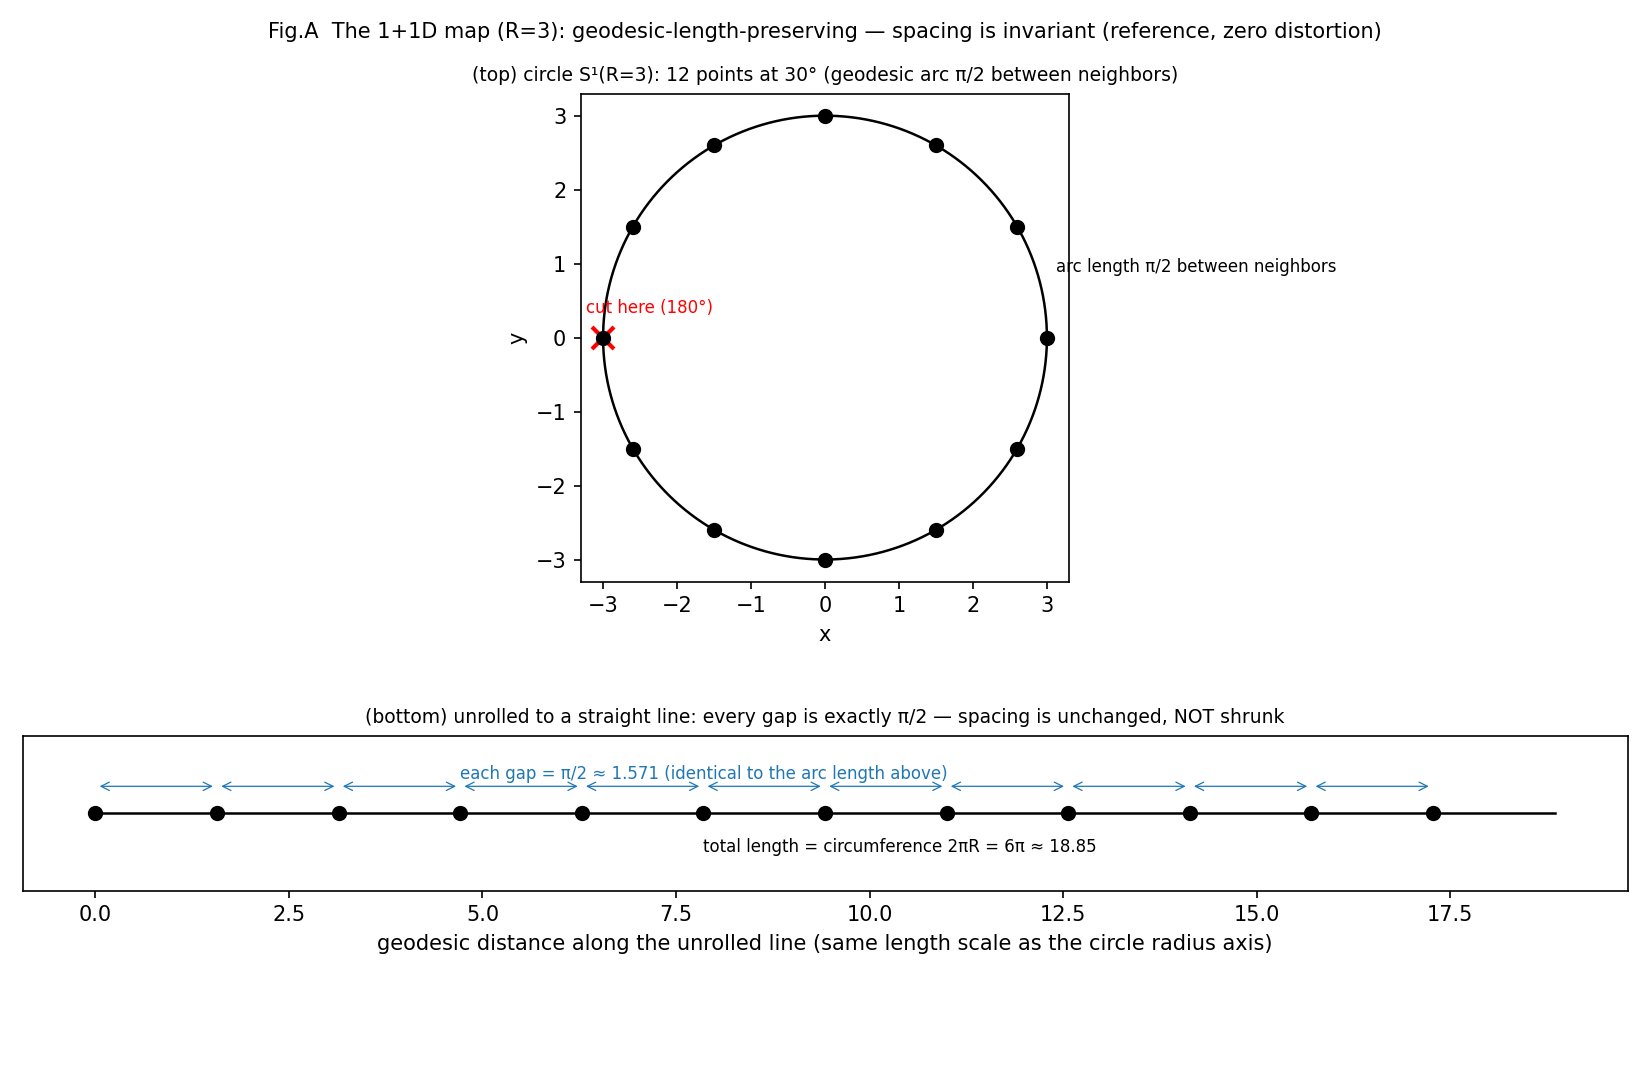
\includegraphics[width=0.88\linewidth,height=\textheight,keepaspectratio]{paper0_figA_1d_reference.png}

\textbf{図A.
1+1次元の写像(R=3、基準像)}。半径3の円周に30°ごとに12点(隣接間の測地距離
π/2)。180°で切って線分に開いても間隔は π/2
のまま------測地線長保存写像では1次元は歪まない。以降の歪みは、この等間隔基準からのズレとして読む。

\subsection{2.
統一体積公式と次元独立な二量}\label{ux7d71ux4e00ux4f53ux7a4dux516cux5f0fux3068ux6b21ux5143ux72ecux7acbux306aux4e8cux91cf}

\textbf{体積(d-content)}:頂点凸包の平坦箱を σ\_R
で写すとヤコビアンが閉じ(§A)、

V\_d(R) = ∫\_\{{[}−t,t{]}\^{}d\} R\^{}d w /
(\textbar y\textbar{}\(^{2}\) + w\(^{2}\))\^{}\{(d+1)/2\} dy. (3)

R→∞ で V\_d→1。d=2 でガウス・ボネ面積と機械精度一致(差 ≤
4×10\(^{-14}\))。

\textbf{頂点角(直角の歪み)---
次元独立}:中心・辺中点・頂点の球面直角三角形にネイピア公式を適用し閉形式化すると、頂点で交わる二辺のなす角
θ は

cos θ(R) = −tan\(^{2}\)(1/2R), すなわち θ(R) =
arccos(−tan\(^{2}\)(1/2R)). (4)

この式に d は現れない。接ベクトルからの数値計算でも d=2〜5
で完全一致を確認した。平坦極限 θ→90° ✓、正曲率で θ\textgreater90°
✓。(等価形 sin(θ/2)=1/(√2 cos(1/2R))。ガウス・ボネとも整合。)

\textbf{2-面の面積(2-content)--- 次元独立}:2-面は辺長 1
の測地正方形であり、球面の\textbf{等質性}(任意位置の合同な測地正方形は同面積)により、その面積はどの次元の超立方体の中でも同一:

A(R) = V\(_{2}\)(R) = R\(^{2}\)(4θ\_rad − 2π) (全 d
で同値、機械確認済み). (5)

\begin{quote}
\textbf{観点の整理(本版の主眼)}:一辺(1-content)・頂点角・2-面の面積(2-content)は、いずれも\textbf{2次元以下の固有量で次元に依らない}。次元
d が効くのは (i) \textbf{存在域}(\(R^{*}_{d}\) が d
とともに上昇)と、(ii) \textbf{体積(d-content)} のみである。
\end{quote}

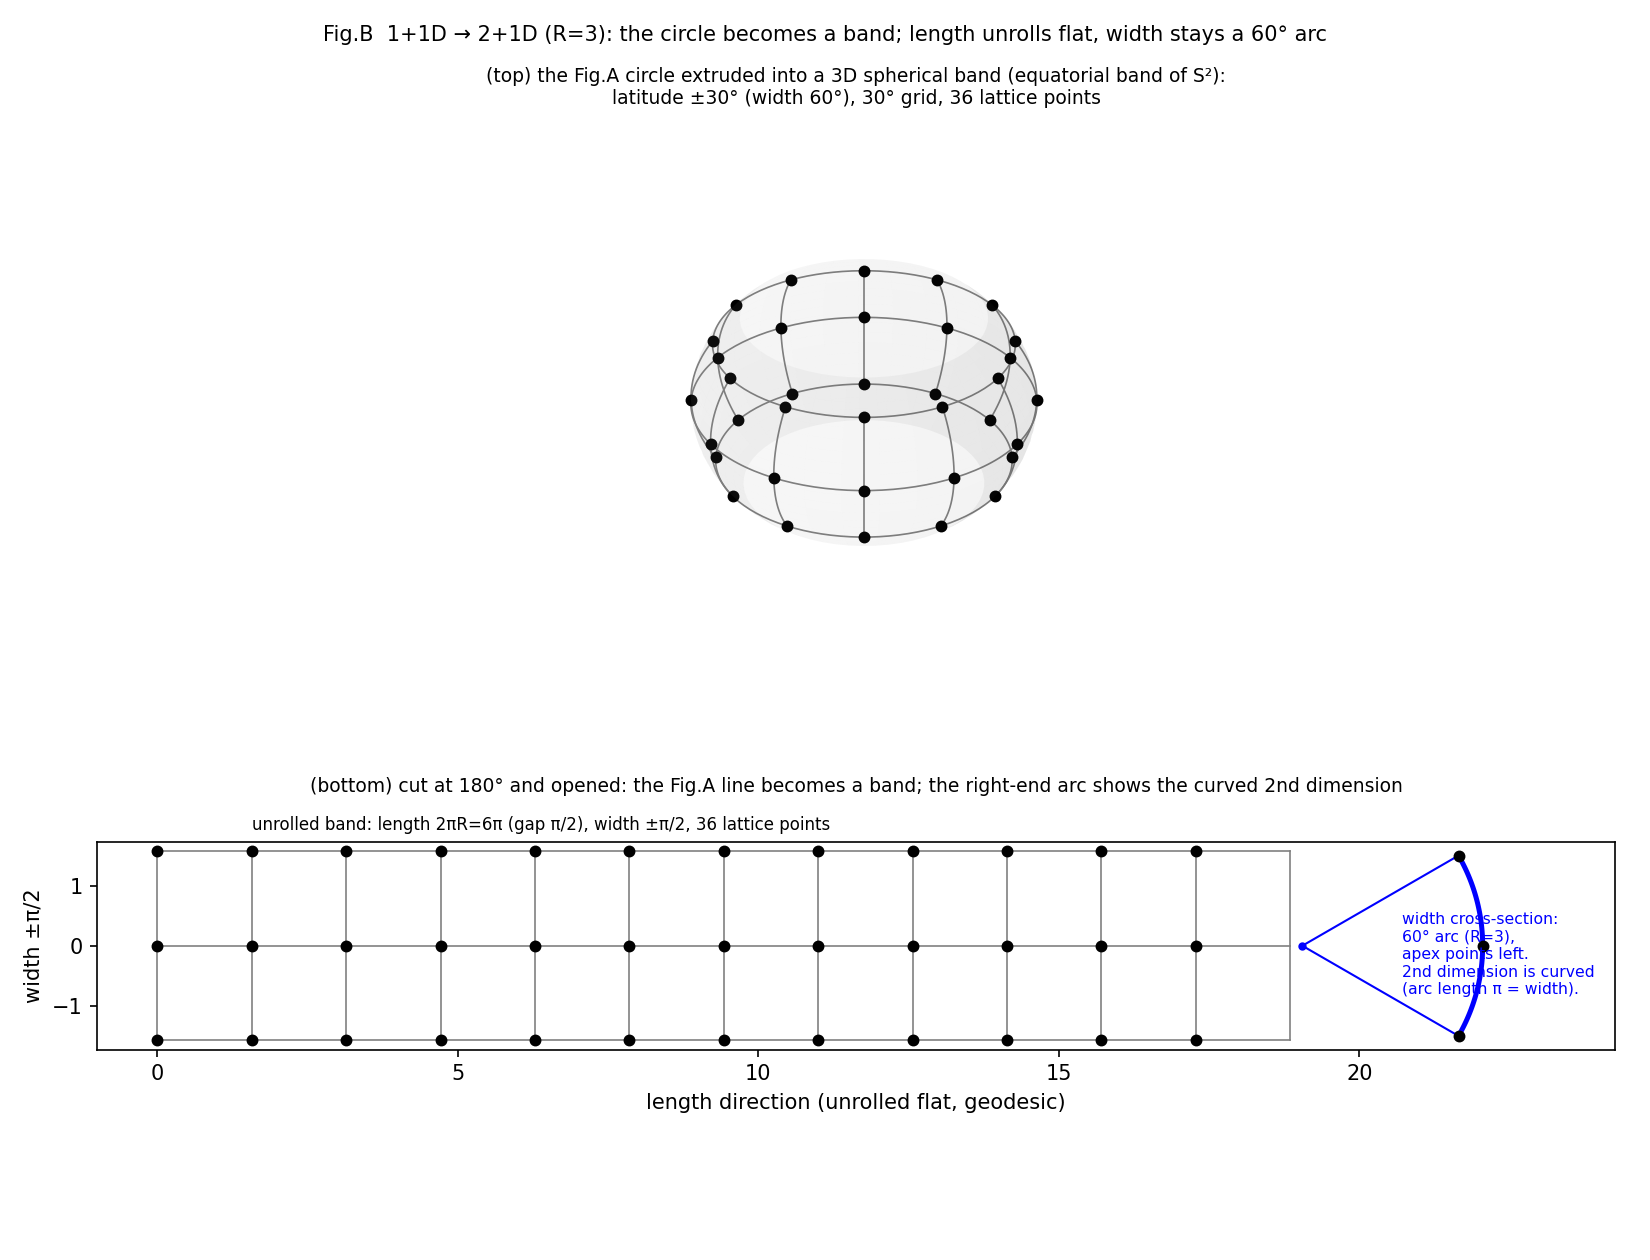
\includegraphics[width=0.88\linewidth,height=\textheight,keepaspectratio]{paper0_figB_band_unfold.png}

\textbf{図B.
1+1→2+1次元の写像(R=3、展開図)}。図Aの円周を緯度±30°(幅60°)の球面帯に拡張(上、30°方眼・36格子点)。180°で切り開くと長さ方向は平らなリボンに開くが(下)、幅方向は60°円弧の断面として曲率を残す(右端の扇形、頂点は左)。長さは平坦に開け幅は曲がる、という非対称が「1次元→2次元」の歪みの芽である。この帯の膨らみ(高さ
h≈0.102)は次元 d によらず同一(§2 次元独立性)。

\subsection{3.
体積の小角係数(次元が効く唯一の量)}\label{ux4f53ux7a4dux306eux5c0fux89d2ux4fc2ux6570ux6b21ux5143ux304cux52b9ux304fux552fux4e00ux306eux91cf}

\begin{enumerate}
\def\labelenumi{(\arabic{enumi})}
\setcounter{enumi}{2}
\tightlist
\item
  を 1/R 展開すると全次元で
\end{enumerate}

V\_d(R) = 1 + c\_d/R\(^{2}\) + O(1/R\(^{4}\)), c\_d = d(d−1)/12 =
C(d,2)/6. (6)

機械検算(R=10\(^{4}\)):d=2〜6 で 1/6, 1/2, 1, 5/3, 5/2 ------すべて
d(d−1)/12 と厳密一致。\textbf{解釈}:d 立方体の体積超過は、その
\textbf{C(d,2) 個の座標2平面それぞれの面積超過(各
1/6=c\(_{2}\))の和}。面積超過 1/6
が「原子」、体積はその一次結合(曲率2形式のトレース)。これが §2
の「面積は次元独立、体積だけ次元依存」の定量形である。

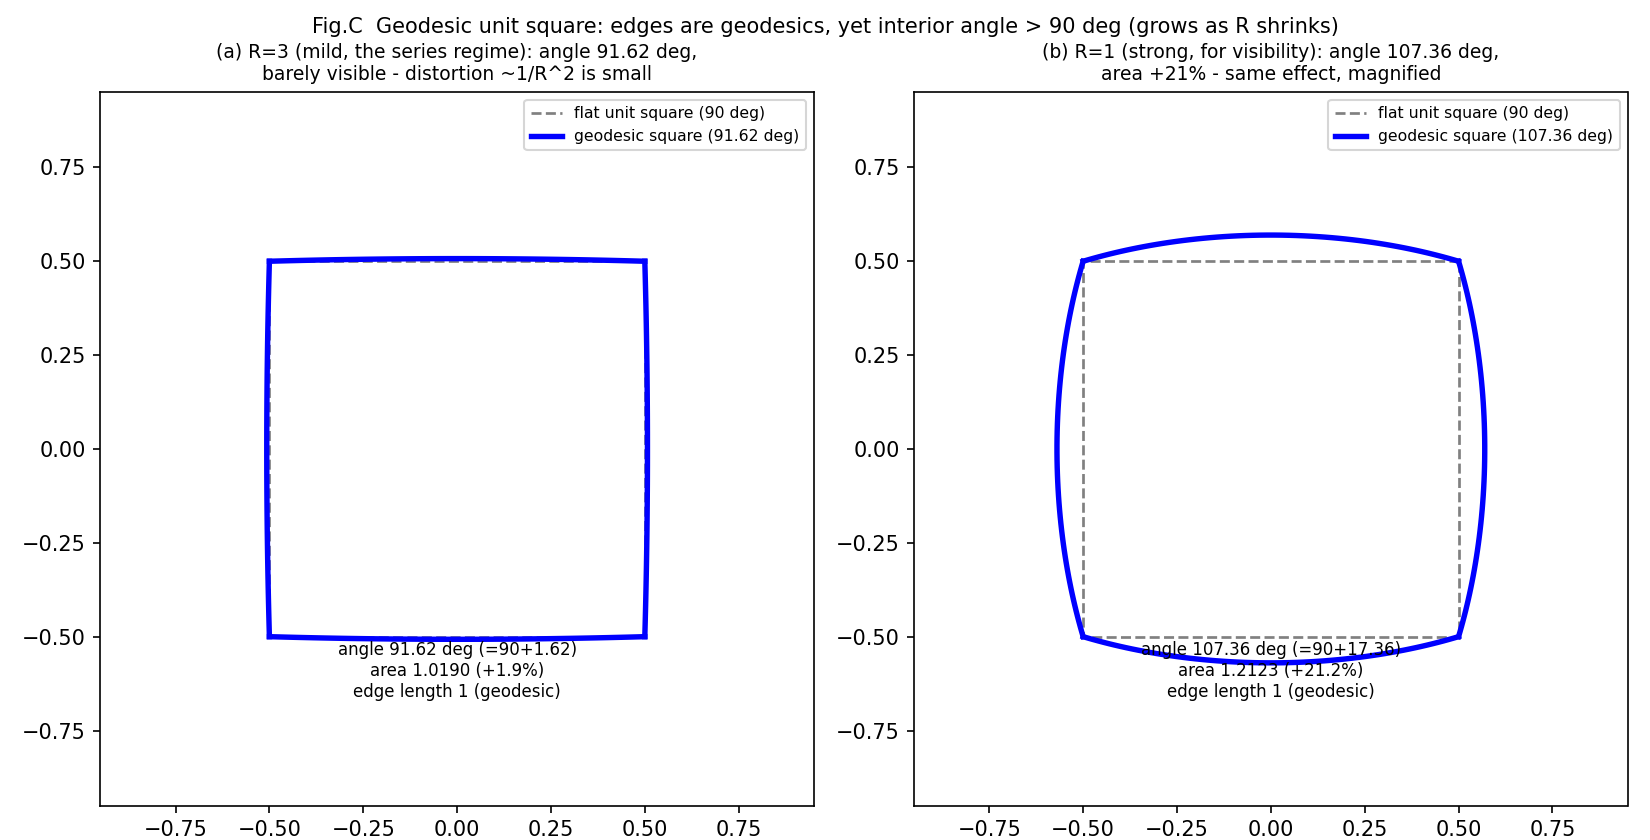
\includegraphics[width=0.88\linewidth,height=\textheight,keepaspectratio]{paper0_figC_angle_excess.png}

\textbf{図C.
測地正方形の角超過}。辺長1の測地正方形(各辺は測地線=その空間の直線)でありながら内角は90°を超える。左:R=3(シリーズの領域、91.62°でほぼ平坦、歪み∝1/R\(^{2}\)は小さい)、右:R=1(視認用、107.36°・面積+21\%、同じ効果が拡大)。歪みは辺長でなく角と面積に現れ、R
が小さいほど大きい。

\subsection{4.
観点別の数表(機械計算・確定値)}\label{ux89b3ux70b9ux5225ux306eux6570ux8868ux6a5fux68b0ux8a08ux7b97ux78baux5b9aux5024}

n/a=存在閾値 (2) 未満。「---」=その次元に当該量が定義されない。

\subsubsection{表1:一辺の長さ(1-content)}\label{ux88681ux4e00ux8fbaux306eux9577ux30551-content}

{\def\LTcaptype{none} % do not increment counter
\begin{longtable}[]{@{}
  >{\raggedright\arraybackslash}p{(\linewidth - 10\tabcolsep) * \real{0.1667}}
  >{\raggedright\arraybackslash}p{(\linewidth - 10\tabcolsep) * \real{0.1667}}
  >{\raggedright\arraybackslash}p{(\linewidth - 10\tabcolsep) * \real{0.1667}}
  >{\raggedright\arraybackslash}p{(\linewidth - 10\tabcolsep) * \real{0.1667}}
  >{\raggedright\arraybackslash}p{(\linewidth - 10\tabcolsep) * \real{0.1667}}
  >{\raggedright\arraybackslash}p{(\linewidth - 10\tabcolsep) * \real{0.1667}}@{}}
\toprule\noalign{}
\begin{minipage}[b]{\linewidth}\raggedright
\end{minipage} & \begin{minipage}[b]{\linewidth}\raggedright
d=1
\end{minipage} & \begin{minipage}[b]{\linewidth}\raggedright
d=2
\end{minipage} & \begin{minipage}[b]{\linewidth}\raggedright
d=3
\end{minipage} & \begin{minipage}[b]{\linewidth}\raggedright
d=4
\end{minipage} & \begin{minipage}[b]{\linewidth}\raggedright
d=5
\end{minipage} \\
\midrule\noalign{}
\endhead
\bottomrule\noalign{}
\endlastfoot
全 R(存在域内) & 1.000000 & 1.000000 & 1.000000 & 1.000000 & 1.000000 \\
\end{longtable}
}

測地線長保存により、一辺は全次元・全 R で厳密に 1(歪みなし)。

\subsubsection{\texorpdfstring{表2:頂点角 θ\href{直角=90°の歪み}{度}---
d=2〜5
で同値}{表2:頂点角 θ度--- d=2〜5 で同値}}\label{ux88682ux9802ux70b9ux89d2-ux3b8ux5ea6-d25-ux3067ux540cux5024}

{\def\LTcaptype{none} % do not increment counter
\begin{longtable}[]{@{}llllll@{}}
\toprule\noalign{}
R & d=1 & d=2 & d=3 & d=4 & d=5 \\
\midrule\noalign{}
\endhead
\bottomrule\noalign{}
\endlastfoot
0.5 & --- & n/a & n/a & n/a & n/a \\
1.0 & --- & 107.36431 & 107.36431 & 107.36431 & n/a \\
1.5 & --- & 96.88584 & 96.88584 & 96.88584 & 96.88584 \\
2.0 & --- & 93.73831 & 93.73831 & 93.73831 & 93.73831 \\
2.5 & --- & 92.35502 & 92.35502 & 92.35502 & 92.35502 \\
3.0 & --- & 91.62171 & 91.62171 & 91.62171 & 91.62171 \\
3.5 & --- & 91.18548 & 91.18548 & 91.18548 & 91.18548 \\
4.0 & --- & 90.90469 & 90.90469 & 90.90469 & 90.90469 \\
5.0 & --- & 90.57681 & 90.57681 & 90.57681 & 90.57681 \\
6.0 & --- & 90.39974 & 90.39974 & 90.39974 & 90.39974 \\
7.0 & --- & 90.29332 & 90.29332 & 90.29332 & 90.29332 \\
8.0 & --- & 90.22440 & 90.22440 & 90.22440 & 90.22440 \\
9.0 & --- & 90.17720 & 90.17720 & 90.17720 & 90.17720 \\
10.0 & --- & 90.14348 & 90.14348 & 90.14348 & 90.14348 \\
100 & --- & 90.00143 & 90.00143 & 90.00143 & 90.00143 \\
1000 & --- & 90.00001 & 90.00001 & 90.00001 & 90.00001 \\
10000 & --- & 90.00000 & 90.00000 & 90.00000 & 90.00000 \\
\end{longtable}
}

直角からの超過 Δθ=θ−90°(度、d非依存):R=1.0 で 17.36°、R=1.5 で
6.89°、R=2 で 3.74°、R=3 で 1.62°、R=5 で 0.577°、R=10 で 0.143°、R=100
で 0.00143°。1/R\(^{2}\) で減衰。

\subsubsection{表3:2-面の面積 A(2-content)--- d=2〜5
で同値(等質性)}\label{ux886832-ux9762ux306eux9762ux7a4d-a2-content-d25-ux3067ux540cux5024ux7b49ux8ceaux6027}

{\def\LTcaptype{none} % do not increment counter
\begin{longtable}[]{@{}llllll@{}}
\toprule\noalign{}
R & d=1 & d=2 & d=3 & d=4 & d=5 \\
\midrule\noalign{}
\endhead
\bottomrule\noalign{}
\endlastfoot
0.5 & --- & n/a & n/a & n/a & n/a \\
1.0 & --- & 1.2122579 & 1.2122579 & 1.2122579 & n/a \\
1.5 & --- & 1.0816255 & 1.0816255 & 1.0816255 & 1.0816255 \\
2.0 & --- & 1.0439325 & 1.0439325 & 1.0439325 & 1.0439325 \\
2.5 & --- & 1.0275733 & 1.0275733 & 1.0275733 & 1.0275733 \\
3.0 & --- & 1.0189503 & 1.0189503 & 1.0189503 & 1.0189503 \\
4.0 & --- & 1.0105516 & 1.0105516 & 1.0105516 & 1.0105516 \\
5.0 & --- & 1.0067216 & 1.0067216 & 1.0067216 & 1.0067216 \\
6.0 & --- & 1.0046561 & 1.0046561 & 1.0046561 & 1.0046561 \\
7.0 & --- & 1.0034156 & 1.0034156 & 1.0034156 & 1.0034156 \\
8.0 & --- & 1.0026125 & 1.0026125 & 1.0026125 & 1.0026125 \\
9.0 & --- & 1.0020628 & 1.0020628 & 1.0020628 & 1.0020628 \\
10.0 & --- & 1.0016701 & 1.0016701 & 1.0016701 & 1.0016701 \\
100 & --- & 1.0000167 & 1.0000167 & 1.0000167 & 1.0000167 \\
1000 & --- & 1.0000002 & 1.0000002 & 1.0000002 & 1.0000002 \\
10000 & --- & 1.0000000 & 1.0000000 & 1.0000000 & 1.0000000 \\
\end{longtable}
}

平坦単位正方形(面積1)からの超過は A−1 ≈ 1/(6R\(^{2}\))。R=3
で約1.9\%増。

\subsubsection{表4:体積 V\_d(d-content)---
次元で真に異なる唯一の量}\label{ux88684ux4f53ux7a4d-v_dd-content-ux6b21ux5143ux3067ux771fux306bux7570ux306aux308bux552fux4e00ux306eux91cf}

{\def\LTcaptype{none} % do not increment counter
\begin{longtable}[]{@{}llllll@{}}
\toprule\noalign{}
R & d=1 & d=2 & d=3 & d=4 & d=5 \\
\midrule\noalign{}
\endhead
\bottomrule\noalign{}
\endlastfoot
0.5 & 1.000000 & n/a & n/a & n/a & n/a \\
1.0 & 1.000000 & 1.2122579 & 1.9499111 & 5.4161376 & n/a \\
1.5 & 1.000000 & 1.0816255 & 1.2801348 & 1.6834544 & 2.5128373 \\
2.0 & 1.000000 & 1.0439325 & 1.1413925 & 1.3119759 & 1.5924206 \\
2.5 & 1.000000 & 1.0275733 & 1.0864041 & 1.1834234 & 1.3302164 \\
3.0 & 1.000000 & 1.0189503 & 1.0585685 & 1.1219513 & 1.2139814 \\
3.5 & 1.000000 & 1.0138368 & 1.0424191 & 1.0873448 & 1.1510492 \\
4.0 & 1.000000 & 1.0105516 & 1.0321808 & 1.0657975 & 1.1127589 \\
4.5 & 1.000000 & 1.0083144 & 1.0252687 & 1.0514201 & 1.0875871 \\
5.0 & 1.000000 & 1.0067216 & 1.0203771 & 1.0413269 & 1.0700953 \\
6.0 & 1.000000 & 1.0046561 & 1.0140697 & 1.0284116 & 1.0479269 \\
7.0 & 1.000000 & 1.0034156 & 1.0103013 & 1.0207484 & 1.0348864 \\
8.0 & 1.000000 & 1.0026125 & 1.0078694 & 1.0158237 & 1.0265506 \\
9.0 & 1.000000 & 1.0020628 & 1.0062083 & 1.0124694 & 1.0208927 \\
10.0 & 1.000000 & 1.0016701 & 1.0050232 & 1.0100810 & 1.0168738 \\
100 & 1.000000 & 1.0000167 & 1.0000500 & 1.0001000 & 1.0001667 \\
1000 & 1.000000 & 1.0000002 & 1.0000005 & 1.0000010 & 1.0000017 \\
10000 & 1.000000 & 1.0000000 & 1.0000000 & 1.0000000 & 1.0000000 \\
\end{longtable}
}

(d=1 は線分=局所平坦で V\(_{1}\)=1。d≥2 で超過
c\_d/R\(^{2}\)、c\_d=1/6,1/2,1,5/3。)

\textbf{極限検算(合格)}:R=100/1000/10000 で全量が平坦値へ 1/R\(^{2}\)
減衰(100\(^{2}\)倍ごと)。全 R で V\_d\textgreater1,
θ\textgreater90°(正曲率の単調超過)。

\subsection{4.5 角度からの曲率の逆算 ---
内部観測者の曲率計}\label{ux89d2ux5ea6ux304bux3089ux306eux66f2ux7387ux306eux9006ux7b97-ux5185ux90e8ux89b3ux6e2cux8005ux306eux66f2ux7387ux8a08}

§2 で頂点角は次元独立な量 cos θ=−tan\(^{2}\)(1/2R) であり、§4 表2
のとおり d=2〜5 で同値だった。ここから重要な帰結が従う:\textbf{d≥2
であれば角度が測れるので、そこから曲率半径 R(より本質的には曲率
K=1/R\(^{2}\))を逆算できる}。これは内部観測者(埋め込みを見られない観測者)にとって、\textbf{曲率の「方向」は不可知だが「値」は可知}であることを意味する。

\subsubsection{負曲率への拡張}\label{ux8ca0ux66f2ux7387ux3078ux306eux62e1ux5f35}

球面(正曲率 K=+1/R\(^{2}\))の解析接続として、双曲空間(負曲率
K=−1/R\(^{2}\))では sin→sinh となり、双曲面模型(Minkowski
計量)での接ベクトル計算から

cos θ(R) = +tanh\(^{2}\)(1/2R)(負曲率、θ \textless{} 90°、全 d
で次元独立、機械確認済み). (8)

\textbf{正負の非対称性(指摘A)}:双曲空間では t=R sinh(1/2R)、w=R√(1+d
sinh\(^{2}\)(1/2R)) であり、根号内は常に正------\textbf{辺長 1
のセルに存在閾値はなく、全 R・全 d で構成可能}(機械確認)。正曲率が
\(R^{*}_{d}\)=1/(2 arcsin(1/√d)) でセルが赤道に達して消える(§1
(2))のと対照的である。負曲率の表(θ=84°→R=1.49
等)はこの無閾値性の下で全域定義される。

正曲率 (4) と並べると、\textbf{頂点角の符号が曲率の符号を決める}:

{\def\LTcaptype{none} % do not increment counter
\begin{longtable}[]{@{}llll@{}}
\toprule\noalign{}
頂点角 & 曲率 & 空間 & 関係式 \\
\midrule\noalign{}
\endhead
\bottomrule\noalign{}
\endlastfoot
θ \textgreater{} 90°(直角超過) & K \textgreater{} 0 & 球面型 & cos θ =
−tan\(^{2}\)(1/2R) \\
θ = 90°(直角) & K = 0 & 平坦 & --- \\
θ \textless{} 90°(直角不足) & K \textless{} 0 & 双曲型 & cos θ =
+tanh\(^{2}\)(1/2R) \\
\end{longtable}
}

すなわち、\textbf{もし角度が90度より小さければ曲率が負}であることが分かる。直角からの偏差
Δθ=θ−90° の符号が、そのまま曲率の符号である。

\subsubsection{逆算公式(曲率計)}\label{ux9006ux7b97ux516cux5f0fux66f2ux7387ux8a08}

辺長を単位 a=1 に正規化すると、測定した頂点角 θ
から曲率と半径が一意に復元される:

θ \textgreater{} 90°: R = 1/(2 arctan√(−cos θ)), K = +1/R\(^{2}\) θ
\textless{} 90°: R = 1/(2 artanh√(+cos θ)), K = −1/R\(^{2}\) (9)

往復検算(R→θ→逆算R)は正・負両曲率・R=1.5〜100
で機械精度一致。逆算の数値例:

{\def\LTcaptype{none} % do not increment counter
\begin{longtable}[]{@{}llll@{}}
\toprule\noalign{}
測定 θ{[}度{]} & 曲率 K & 半径 R & 種別 \\
\midrule\noalign{}
\endhead
\bottomrule\noalign{}
\endlastfoot
84.0 & −0.449805 & 1.49103 & 負(双曲型) \\
88.0 & −0.142935 & 2.64503 & 負(双曲型) \\
89.5 & −0.035111 & 5.33680 & 負(双曲型) \\
90.0 & 0 & ∞ & 平坦 \\
90.5 & +0.034704 & 5.36794 & 正(球面型) \\
92.0 & +0.136435 & 2.70731 & 正(球面型) \\
96.0 & +0.391129 & 1.59897 & 正(球面型) \\
107.36431 & +1.000000 & 1.00000 & 正(球面型) \\
\end{longtable}
}

\subsubsection{意味(シリーズの主題との接続)}\label{ux610fux5473ux30b7ux30eaux30fcux30baux306eux4e3bux984cux3068ux306eux63a5ux7d9a}

\begin{enumerate}
\def\labelenumi{(\roman{enumi})}
\item
  \textbf{次元普遍性}:角度の逆算式 (9) には d
  が現れない。2次元の観測者も4次元の観測者も、局所の頂点角を測れば\textbf{同じ
  K} を得る------曲率計は次元を問わない。
\item
  \textbf{方向は不可視、値は可知}:内部観測者は曲率の「向き」(埋め込みでどちらに反るか、極の位置=マーキング)を知り得ない。それはゲージ(不可視方向)である。しかし曲率スカラー
  K(符号と大きさ)は、\textbf{たった一つの局所角度測定}から完全に決まる。これは本シリーズ本体で
  R・Q
  が全マーキング共有の不変量であり、どの軸が時間か(向き)はゲージである構造(論文14
  マーキング定理)と同型の図式である。
\item
  \textbf{d=1 では測れない}:1次元には頂点角がなく(辺のみ)、曲率計は d≥2
  を要する。これは「歪みは d≥2 で初めて発生する」(初出の根拠は §1〜2:d=1
  は内在的平坦で歪みゼロ;まとめは §7)の観測的側面である。
\end{enumerate}

\subsection{4.6
次元の曖昧さと次元の共役量(観察)}\label{ux6b21ux5143ux306eux66d6ux6627ux3055ux3068ux6b21ux5143ux306eux5171ux5f79ux91cfux89b3ux5bdf}

§1 の存在条件 d·sin\(^{2}\)(1/2R) ≤ 1
を\textbf{次元について解く}と、与えられた曲率半径 R で辺長 1
の正則測地セルが収まる\textbf{最大次元}が出る:

\(d_{\max}(R) = \lfloor 1/\sin^2(1/2R)\rfloor = \lfloor \csc^2(1/2R)\rfloor \approx 4R^2\)（大
R 漸近）、\(R \ge 1/\pi\). (10)

つまり\textbf{次元は曲率によって上から抑えられている}。許される次元は
\{1, 2, \ldots, d\_max(R)\}
の範囲にあり、一意には決まらない------\textbf{与えられた R
に対して次元には曖昧さがある}。

\subsubsection{次元の曖昧さは小 R
で(相対的に)増える}\label{ux6b21ux5143ux306eux66d6ux6627ux3055ux306fux5c0f-r-ux3067ux76f8ux5bfeux7684ux306bux5897ux3048ux308b}

R の不確定性 ±½(§6)を伝播させると、天井 d\_max 自体が幅を持つ:

{\def\LTcaptype{none} % do not increment counter
\begin{longtable}[]{@{}
  >{\raggedright\arraybackslash}p{(\linewidth - 10\tabcolsep) * \real{0.1667}}
  >{\raggedright\arraybackslash}p{(\linewidth - 10\tabcolsep) * \real{0.1667}}
  >{\raggedright\arraybackslash}p{(\linewidth - 10\tabcolsep) * \real{0.1667}}
  >{\raggedright\arraybackslash}p{(\linewidth - 10\tabcolsep) * \real{0.1667}}
  >{\raggedright\arraybackslash}p{(\linewidth - 10\tabcolsep) * \real{0.1667}}
  >{\raggedright\arraybackslash}p{(\linewidth - 10\tabcolsep) * \real{0.1667}}@{}}
\toprule\noalign{}
\begin{minipage}[b]{\linewidth}\raggedright
R
\end{minipage} & \begin{minipage}[b]{\linewidth}\raggedright
κ=sin\(^{2}\)(1/2R)
\end{minipage} & \begin{minipage}[b]{\linewidth}\raggedright
d\_max(R−½)
\end{minipage} & \begin{minipage}[b]{\linewidth}\raggedright
d\_max(R)
\end{minipage} & \begin{minipage}[b]{\linewidth}\raggedright
d\_max(R+½)
\end{minipage} & \begin{minipage}[b]{\linewidth}\raggedright
相対幅 Δd/d
\end{minipage} \\
\midrule\noalign{}
\endhead
\bottomrule\noalign{}
\endlastfoot
0.5 & 0.708073 & 0 & 1 & 4 & 3.000 \\
0.7 & 0.429127 & 0 & 2 & 6 & 2.500 \\
1.0 & 0.229849 & 1 & 4 & 9 & 2.000 \\
1.5 & 0.107056 & 4 & 9 & 16 & 1.333 \\
2.0 & 0.061209 & 9 & 16 & 25 & 1.000 \\
3.0 & 0.027522 & 25 & 36 & 49 & 0.667 \\
5.0 & 0.009967 & 81 & 100 & 121 & 0.400 \\
10.0 & 0.002498 & 361 & 400 & 441 & 0.200 \\
\end{longtable}
}

(d\_max=0 は R\textless1/π≈0.318 の前幾何領域=構造のない点、§4.7
と統一。)

\textbf{相対的な次元の曖昧さ Δd/d は R が小さいほど大きい}(R=1 で d\_max
は 1〜9 と振れる)。R が小さい領域では ±½
が相対的に巨大なので、次元が鋭く決まらない。逆に大
R(平坦近く)では天井は高い(d\_max≈4R\(^{2}\))が、相対幅は 1/R
で縮み次元は安定する。二つの読みが同居する:\textbf{強曲率は絶対的な天井を下げ(次元を低く制限)、同時に
±½ ゆらぎ下での相対的曖昧さを上げる}。

\subsubsection{次元の共役量の候補}\label{ux6b21ux5143ux306eux5171ux5f79ux91cfux306eux5019ux88dc}

\begin{enumerate}
\def\labelenumi{(\arabic{enumi})}
\setcounter{enumi}{9}
\tightlist
\item
  は容量関係 \textbf{d·κ ≤ 1}(κ ≡ sin\(^{2}\)(1/2R)、予算
  1)と書ける。飽和 d·κ=1 がちょうど天井 \(R^{*}_{d}\)(d=2〜5 で 10
  桁一致を確認)。残容量は幾何学的に
\end{enumerate}

1 − d·κ =
(w/R)\(^{2}\)(セル中心の極余緯度の余弦\(^{2}\)、頂点が赤道に達すると 0).

すなわち\textbf{各空間次元は単位曲率予算から κ
ずつを消費し、予算を使い切ると次元の天井に達する}。大 R 漸近で κ ≈
1/(4R\(^{2}\)) = K/4(K=1/R\(^{2}\) は曲率)であり、

d × (K/4) ≲ 1, すなわち 次元 ≲ 4/曲率.

(橋渡し:K=1/R\(^{2}\) なので
4/K=4R\(^{2}\)。よって「d\_max≈4R\(^{2}\)(大 R、§4.6
冒頭)」と「d·(K/4)≲1」は同一の関係の二表記である。)

\begin{quote}
\textbf{観察(本稿の主張ではなく問題提起)}:設計者の問い「次元の共役量は何か」に対する幾何学的候補は、\textbf{1軸あたり曲率負荷
κ=sin\(^{2}\)(1/2R)(≈ 曲率/4)} である。次元 d と κ
は容量共役(d·κ≤1)をなし、νλ=1 や
Σν\(^{2}\)=\(\mathcal{N}\)\(^{2}\)(論文1)と同じ「保存予算の飽和」型の関係にある。これは厳密な幾何学的事実(存在条件の言い換え)だが、その\textbf{共役としての解釈は観察であり定理ではない}。物理的同一視は行わない。
\end{quote}

\subsubsection{シリーズへの含意(範囲の明示)}\label{ux30b7ux30eaux30fcux30baux3078ux306eux542bux610fux7bc4ux56f2ux306eux660eux793a}

本シリーズが働く R は小さい(R=1〜3 程度)。そこでは (10) より
d\_max=4〜36 であり、\textbf{次元 4
は幾何学的に許される一つの値にすぎず、幾何だけでは d=4
に固定されない}。d=4 への固定は論文11
の算術的機構(\{1,2,4,8\}∩平方数)によるものであって、本稿の幾何学的曖昧さとは別軸である。本稿が示すのは「幾何は次元に天井と曖昧さを与えるが、特定の次元は選ばない」という、論文11
と相補的な事実である。\textbf{離散系への本格的な接続(次元の不確定性関係の定式化)は本稿の範囲外とし、観察の提示にとどめる。}

\subsubsection{先行研究との関係(差別化)}\label{ux5148ux884cux7814ux7a76ux3068ux306eux95a2ux4fc2ux5deeux5225ux5316}

「次元が一意でなくスケールに依存しうる」という着想自体は新しくない。拡散で測る\textbf{スペクトル次元}は量子重力(因果的動的三角分割・漸近安全性・ループ量子重力)で短距離
∼2・長距離 ∼4 と流れることが知られ {[}Carlip 2017;
Ambjørn--Jurkiewicz--Loll
2005{]}、次元正則化やフラクタル次元も同系である。定曲率空間で\textbf{曲率半径が幾何的限界を半径依存で与える}という点では、\textbf{Böröczky
のパッキング密度上界} {[}Böröczky 1978{]}
が最も近い先例である。本稿が異なるのは三点:(i)
天井の源泉が拡散・密度ではなく「辺長 1
の正則測地セルが整数個収まるか」という\textbf{離散的存在条件}
d·sin\(^{2}\)(1/2R)≤1 であること(存在閾値 R*\_d は球面正多胞体の
Schläfli 的存在条件 {[}Coxeter 1973{]} の系譜に属する)、(ii)
これが\textbf{次元の共役量} κ=sin\(^{2}\)(1/2R) と容量関係 d·κ≤1
として、νλ=1・Σν\(^{2}\)=\(\mathcal{N}\)\(^{2}\)
と同型の保存予算飽和に乗ること、(iii) 幾何天井と論文11
の検閲天井という\textbf{独立2機構が d=4
で臨界一致}すること(§4.7)。すなわち「なぜ4次元か」の議論は古くから多い
{[}Ehrenfest 1917; Tegmark 1997{]}
が、本稿の主張は\textbf{この連鎖の具体性}にあり、「次元の曖昧さ」一般を新概念として主張するものではない。

\subsection{4.7 ゼロ次元からの次元創発と d=4
での安定化(観察)}\label{ux30bcux30edux6b21ux5143ux304bux3089ux306eux6b21ux5143ux5275ux767aux3068-d4-ux3067ux306eux5b89ux5b9aux5316ux89b3ux5bdf}

§4.6 の幾何天井 d\_max(R)≈4R\(^{2}\) は \textbf{R
とともに上昇}する(曲率が弱まると高次元が収まる)。これに論文11
の\textbf{検閲天井}を重ねると、次元の創発と d=4
での安定化が一枚の絵になる。

\subsubsection{二つの天井}\label{ux4e8cux3064ux306eux5929ux4e95}

\begin{itemize}
\tightlist
\item
  \textbf{幾何天井(本稿)}:d\_max(R)=\(\lfloor\)csc\(^{2}\)(1/2R)\(\rfloor\)≈4R\(^{2}\)。R
  が小さい(強曲率)ほど低く、R とともに上昇。
\item
  \textbf{検閲天井(論文11 両端点定理;補遺25-26)}:梯子の曲率歪み
  (√d−1)\(^{2}\)/2(\textbf{この式は論文11
  で導かれたもので、本稿は所与として用いる}------梯子=着衣周波数の対角
  √d に由来、半波長検閲限界 ½ は論文9)が ½ 以下となるのは d ≤ 4
  のみ。\textbf{d=4 はちょうど等号 (√4−1)\(^{2}\)/2=½(臨界)}、d=5 では
  0.764\textgreater½ で検閲され不安定。この天井は R に依らず\textbf{固定
  4}。
\end{itemize}

安定に存在できる次元は両天井の小さい方
\textbf{d\_stable(R)=min(d\_max(R), 4)} である。

\subsubsection{次元の階段(機械計算)}\label{ux6b21ux5143ux306eux968eux6bb5ux6a5fux68b0ux8a08ux7b97}

{\def\LTcaptype{none} % do not increment counter
\begin{longtable}[]{@{}
  >{\raggedright\arraybackslash}p{(\linewidth - 6\tabcolsep) * \real{0.2500}}
  >{\raggedright\arraybackslash}p{(\linewidth - 6\tabcolsep) * \real{0.2500}}
  >{\raggedright\arraybackslash}p{(\linewidth - 6\tabcolsep) * \real{0.2500}}
  >{\raggedright\arraybackslash}p{(\linewidth - 6\tabcolsep) * \real{0.2500}}@{}}
\toprule\noalign{}
\begin{minipage}[b]{\linewidth}\raggedright
R の領域
\end{minipage} & \begin{minipage}[b]{\linewidth}\raggedright
幾何天井 d\_max
\end{minipage} & \begin{minipage}[b]{\linewidth}\raggedright
安定次元 d\_stable
\end{minipage} & \begin{minipage}[b]{\linewidth}\raggedright
状態
\end{minipage} \\
\midrule\noalign{}
\endhead
\bottomrule\noalign{}
\endlastfoot
R \textless{} 1/π≈0.318 & 0 & 0 & 前幾何(点) \\
{[}1/π, 2/π) & 1 & 1 & d=1 \\
{[}2/π, \(R^{*}_{3}\))≈{[}0.637, 0.812) & 2 & 2 & d=2 \\
{[}\(R^{*}_{3}\), 3/π)≈{[}0.812, 0.955) & 3 & 3 & d=3 \\
\textbf{R ≥ 3/π≈0.955} & 4, 9, 16, \ldots(上昇) & \textbf{4(ロック)} &
\textbf{検閲が 4 で上限} \\
\end{longtable}
}

各次元の創発閾値は §1 (2) の \(R^{*}_{d}\)=1/(2 arcsin(1/√d))
そのもの:d=k は R≥\(R^{*}_{k}\) で幾何的に出現する。

\subsubsection{物語:climb して 4
でロック}\label{ux7269ux8a9eclimb-ux3057ux3066-4-ux3067ux30edux30c3ux30af}

\begin{enumerate}
\def\labelenumi{(\roman{enumi})}
\item
  \textbf{ゼロ次元から}:最強曲率(最小 R)では幾何天井が低く、次元は 0〜1
  に抑えられる(構造のない点/線分から始まる)。
\item
  \textbf{次元の創発(階段を登る)}:R が増す(曲率が弱まる=論文8 の内部膨張
  a∝√t に対応しうる)につれ幾何天井 d\_max
  が上昇する。\textbf{ただし創発(実現)するのは安定次元
  d\_stable=min(d\_max, 4) であって、d\_max
  自身は『収まりうる最大次元』の上界が単調上昇するだけである}(d\_max(3)=36
  でも実現は検閲天井で 4)。d\_stable が d=1→2→3→4
  と一段ずつ登るのが創発であり、±½
  により鋭いジャンプでなく曖昧な段(§4.6)になる。
\item
  \textbf{なぜ 4 で止まるか}:R=3/π
  で上昇する幾何天井がちょうど固定の検閲天井 4 に到達する。R
  がさらに増せば幾何的には d=5,6,\ldots{}
  も収まる(d\_max→∞)が、それらは検閲歪み (√d−1)\(^{2}\)/2\textgreater½
  で\textbf{不安定}(論文11)。よって安定次元は 4
  にロックされ、以後どれだけ膨張しても 4 のまま。
\end{enumerate}

\begin{quote}
\textbf{観察(本稿の主張ではなく総合)}:\textbf{d=4
は、上昇する幾何天井と固定の検閲天井が交わる唯一の次元------到達可能でありかつ安定な最後の段}である。しかも
d=4 は検閲歪みがちょうど ½
の\textbf{臨界}点(等号)であり、「最大かつ際どく安定」な次元として選ばれる。ゼロ次元から膨張とともに次元が創発し
4 で安定化する、という描像が、本稿の幾何天井(§4.6)と論文11
の検閲天井の\textbf{二つの独立な機構の合成}として得られる。これは厳密な二事実の総合だが、創発の物理過程としての主張ではない。物理的同一視は行わない。
\end{quote}

\subsubsection{範囲の明示}\label{ux7bc4ux56f2ux306eux660eux793a}

本稿が新たに与えるのは「幾何天井が R
とともに上昇する」という一事実のみで、d=4 の特権性と梯子歪み式
(√d−1)\(^{2}\)/2
は論文11(両端点定理、補遺25-26)が担い、本稿は所与として合成する。両者は独立(一方は曲率半径の幾何、他方は梯子の整数性と検閲)であり、その合致が描像に説得力を与える。膨張
R(t)
の動力学・次元創発の時間発展の定式化は本稿の範囲外とし、観察にとどめる。

\subsection{4.8 1次元論理波の曲率厳密性と論文9
との接続(観察)}\label{ux6b21ux5143ux8ad6ux7406ux6ce2ux306eux66f2ux7387ux53b3ux5bc6ux6027ux3068ux8ad6ux65879-ux3068ux306eux63a5ux7d9aux89b3ux5bdf}

本稿の最初の結果(§2)は \textbf{d=1
の測地セルは内在的平坦------一辺・角・面積・体積すべて歪みゼロ、R
に依らない(R=3 を含む)}
であった。これがシリーズ本体の基礎にどう効くかを明示する。

\subsubsection{シリーズの波は軸ごとに1次元}\label{ux30b7ux30eaux30fcux30baux306eux6ce2ux306fux8ef8ux3054ux3068ux306b1ux6b21ux5143}

論文5 の辞書定理は、数え上げ N\(_{0}\)(R) の波動的正体を「各軸の周波数
m\(_i\) に零点シフト +½
を加えた\textbf{実フーリエ基底の積}」と同定した(軸ごとの多重度パターン
\{1,2,2,\ldots\} は実フーリエ基底そのもの)。すなわち\textbf{波の中身は
per-axis の1次元定在波の積}である。論文2
の数え上げは一辺1の平坦4セル(各体積
1\(^{4}\)=1)の整数格子計数であり、曲面上の測度ではない。論文9 §2.1
の論理波(零点 ½
基底の奇数倍音列、矩形波、位置=位相、平行移動=線形位相乗算)も per-axis
の1次元・縦波的構造である。

\subsubsection{二つの独立な根拠が同じ結論に来る}\label{ux4e8cux3064ux306eux72ecux7acbux306aux6839ux62e0ux304cux540cux3058ux7d50ux8ad6ux306bux6765ux308b}

設計者の主張「R
が小さく(例:R=3)ても、1次元波で振幅が無視できる(矩形波・論理波として振幅を正準化=縦波的に扱える)なら厳密」は、\textbf{独立な二経路}で支持される:

\begin{itemize}
\tightlist
\item
  \textbf{幾何(本稿 §2)}:per-axis の1次元波が住むのは d=1。d=1
  の曲率歪みは\textbf{厳密にゼロ}(任意の
  R)。よって1次元波の平坦扱いは近似でなく厳密。
\item
  \textbf{エネルギー(論文9 §2.3「曲率整合」)}:論文9 §2.3
  は「振幅は伝播方向の外への変位であり、その二乗の局所エネルギー密度が局所曲率と結合して自己相互作用する。位相のみの波(±1
  値)は局所エネルギー密度が一様で、線形位相計算が厳密のまま生き残る」と述べる(引用は論文9
  §2.3 原文の趣旨;本稿はこれを所与として幾何側 d=1=0 と並置する)。
\end{itemize}

幾何(d=1=歪みゼロ)とエネルギー(振幅なし=曲率非結合)は別の理屈だが、\textbf{同一の対象(振幅なし1次元論理波)の曲率厳密性が二面で整合的に確認される}(同一対象の二側面であって、独立な二命題の偶然の一致ではない)。論文0
はこの収束に、論文9
が定性的に述べた「曲率整合」の\textbf{定量的・幾何学的根拠}(d=1 で
c\_d=0、d≥2 で初めて c\_d=d(d−1)/12\textgreater0)を与える。

\subsubsection{読みの非一意性は §4.6
の次元曖昧さの別表現}\label{ux8aadux307fux306eux975eux4e00ux610fux6027ux306f-4.6-ux306eux6b21ux5143ux66d6ux6627ux3055ux306eux5225ux8868ux73fe}

注意すべきは、\textbf{同一の N\(_{0}\)(R)
セルが二通りに読める}ことである:per-axis
の1次元読み(c\(_{1}\)=0、補正なし)と、d
次元結合読み(c\_d\textgreater0、例えば d=4 で
12\%超過)。どちらが正しい読みかは論文0
単独では決まらない------これは欠陥ではなく、\textbf{§4.6
の「次元の曖昧さ」の別表現}である:同一セルの per-axis 1次元読みと d
次元結合読みは両立する別の射影であり、どちらを取るかが次元の曖昧さに対応する。シリーズは前者(平坦格子+per-axis
1次元、論文2・5・9)を構成上採る。本稿はこの選択を正当化するのでなく、二つの読みが共存することと、シリーズの選択がどちらかを明示する。

\subsubsection{含意:歪みの座は
d≥2、そこを論理波が回避する}\label{ux542bux610fux6b6aux307fux306eux5ea7ux306f-d2ux305dux3053ux3092ux8ad6ux7406ux6ce2ux304cux56deux907fux3059ux308b}

本稿 §3〜4 の歪み(c\_d\textgreater0)は \textbf{d≥2
の真の測地胞体(頂点角を持つ結合幾何)}
にのみ現れる。シリーズは、計数を平坦格子で(論文2)・波を per-axis
1次元で(論文5)・振幅を正準化して(論文9)扱うことで、\textbf{歪みの座(d≥2
結合幾何)を構成上回避し、曲率厳密な領域に留まっている}。これは設計者の主張の幾何基礎での裏打ちであり、同時に「論文0
がシリーズに対して持つ意味」の正確な記述である:\textbf{論文0
は平坦扱いの不足を補うのではなく、平坦扱いが厳密に成立する範囲を画定し、それが論理波の住む範囲と一致することを示す}。物理的同一視は行わない。

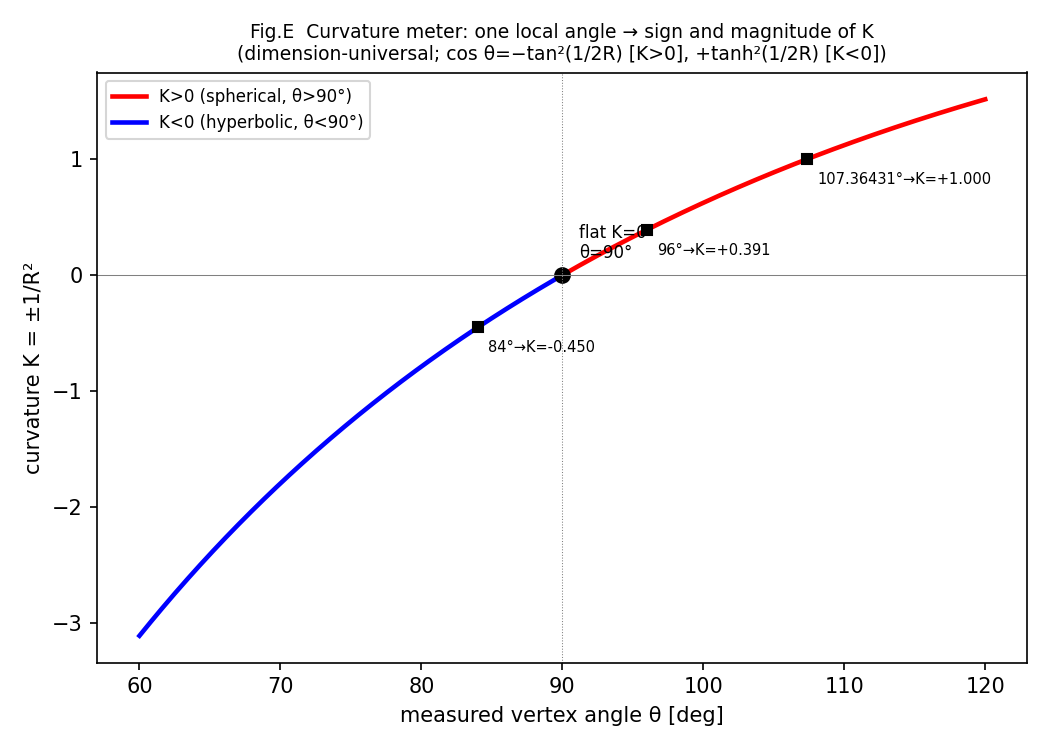
\includegraphics[width=0.88\linewidth,height=\textheight,keepaspectratio]{paper0_figE_curvature_meter.png}

\textbf{図E. 曲率計(§4.5)}。測定した頂点角 θ から曲率 K
を逆算する一本の曲線。θ\textless90°でK\textless0(双曲)、θ=90°でK=0(平坦)、θ\textgreater90°でK\textgreater0(球面)。逆算例(84°→K=−0.45
等)が曲線上に乗る。式に d
が現れず次元普遍------内部観測者は曲率の方向(マーキング)を知り得ないが、局所角度ひとつから
K の符号と大きさを読める。

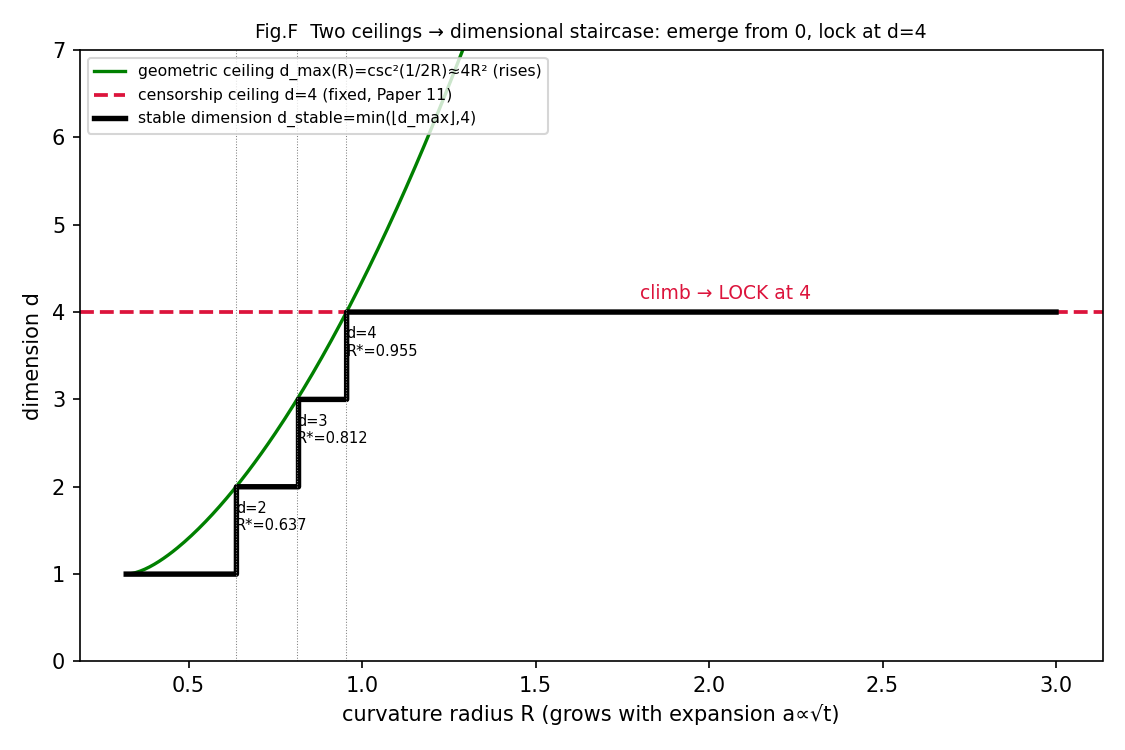
\includegraphics[width=0.88\linewidth,height=\textheight,keepaspectratio]{paper0_figF_staircase.png}

\textbf{図F. 次元の階段(§4.7)}。上昇する幾何天井
d\_max(R)≈4R\(^{2}\)(緑)と固定の検閲天井
d=4(赤破線、論文11)の小さい方が安定次元(太線)。R の増大(膨張)とともに
1→2→3→4 と登り、R≥3/π で 4 にロックする。

\subsection{5. 論文1・2
との接続}\label{ux8ad6ux658712-ux3068ux306eux63a5ux7d9a}

論文2 の平坦数え上げは各セルに超体積 1
を割り当てた。曲率補正の主項を\textbf{平均場近似}(全セルに一律
V\(_{4}\)(R) 倍を割り当てる近似)で見積もると

ΔN(R) ≈ N\(_{0}\)(R)·(V\(_{4}\)(R) − 1) = N\(_{0}\)(R)/R\(^{2}\) +
O(1/R\(^{4}\))(平均場). (11)

R が小さいほど 1/R\(^{2}\) で大きく効き、R→∞ で消える。R=3 で
V\(_{4}\)=1.1220(約12\%超過)。

\begin{quote}
\textbf{平均場近似であることの明示(査読者の設計意図確認への回答)}:(11)
は各セルを「極中心の測地単位超立方体」とみなし一律 V\(_{4}\)(R)
倍する近似である。球面の等質性により\textbf{極中心の測地セルの体積は位置に依らず
V\(_{4}\)(R)} だが、論文1〜2 の実際の格子セルは制約面
Σν\(^{2}\)=R\(^{2}\) に対して様々な向き・位置(極からの測地距離
χ)で乗っており、向き付きの超過率はセルごとに異なりうる。したがって (11)
は\textbf{指導的(leading-order)・平均場の見積もり}であり、\textbf{殻位置・向き依存を解像した厳密版は将来課題}とする。また制約面の次元(4D
周波数空間では Σ\_\{i=1\}\^{}4 ν\(^{2}\)=R\(^{2}\) は S\(^{3}\))と本稿の
S\^{}d(R)
の対応関係の精密化も同枠の将来課題である。本稿が確定したのは「単位測地セルの曲率超過は厳密に
1+c\_d/R\(^{2}\)」までであり、それを数え上げへ移す際の一律倍は近似である。\textbf{なお
(11)
は『セルを多次元測地胞体と読み替えた場合』の見積もりであって、シリーズが実際に扱う
per-axis 1次元論理波+平坦格子計数(§4.8)には d=1
ゆえ補正は要らない(c\(_{1}\)=0)。} よって §5
は仮想的解釈に対する将来課題であり、論文1〜2
の現行内容が曲率で不足しているという含意ではない。
\end{quote}

\subsection{6. R のバラツキ
±½}\label{r-ux306eux30d0ux30e9ux30c4ux30ad-uxbd}

各量を {[}R−½, R+½{]} で評価。d=4 の例(V\(_{4}\)):R=2 で
1.6835/1.3120/1.1834、R=5 で 1.0514/1.0413/1.0340、R=10 で
1.0112/1.0101/1.0091。小 R で幅大(非線形)、大 R で対称・微小。

\subsection{7. 主張範囲}\label{ux4e3bux5f35ux7bc4ux56f2}

主張する:(1) 歪みは d=1 で発生せず、d≥2 で 1/R\(^{2}\)
を主係数として発生。(2) 一辺の測地長は全次元・全 R で不変(1)。(3)
\textbf{頂点角・2-面の面積は次元独立}(2次元固有量、cos
θ=−tan\(^{2}\)(1/2R)、A=V\(_{2}\))。(4)
\textbf{体積のみ次元依存}で係数は閉形式 c\_d=d(d−1)/12(= C(d,2)
個の面積超過の和)。(5) 次元 d
は値でなく存在域(\(R^{*}_{d}\))にも効く。(6) 超過 (11)
は多次元測地胞体への読み替えに対する平坦数え上げの曲率補正主項(平均場、§5)。(7)
\textbf{per-axis 1次元論理波(論文5・9)は d=1 ゆえ曲率厳密(歪みゼロ、任意
R)}------論文9 §2.3「曲率整合」の幾何的根拠(§4.8)。シリーズは歪みの座
d≥2 を構成上回避している。(7)
\textbf{角度から曲率の符号と大きさが次元普遍に逆算できる}(曲率計、§4.5):θ\textgreater90°\(\Longrightarrow\)K\textgreater0、θ\textless90°\(\Longrightarrow\)K\textless0。方向(マーキング)は不可知だが値
K は局所角度から可知。(8) \textbf{次元には天井
d\_max(R)=\(\lfloor\)csc\(^{2}\)(1/2R)\(\rfloor\)≈4R\(^{2}\)
と曖昧さがあり}、±½ 下の相対曖昧さは小 R
で増大(§4.6)。次元の共役量の候補は1軸あたり曲率負荷
κ=sin\(^{2}\)(1/2R)≈K/4(d·κ≤1、観察)。(9) \textbf{二つの天井(幾何
d\_max(R)↑ と検閲 4 固定)の合成}で、ゼロ次元から次元が創発し d=4
でロックする階段が得られる(§4.7、観察)。

主張しない:物理的同一視/測度・確率・振幅(本稿に存在しない)。

\subsection{付録A:ヤコビアンの導出(体積公式
(3))}\label{ux4ed8ux9332aux30e4ux30b3ux30d3ux30a2ux30f3ux306eux5c0eux51faux4f53ux7a4dux516cux5f0f-3}

\(f(y)=R(y,w)/\sqrt{|y|^2+w^2}\)、\(r=\sqrt{|y|^2+w^2}\) とおく。すると
\(\partial f/\partial y_j=(R/r)\,[\,e_j^{(d+1)} - (y,w)\,y_j/r^2\,]\)。グラム行列
\(G=J^{T}J\) は
\(G_{ij}=(R/r)^2[\,\delta_{ij} - y_i y_j/r^2\,]\)、\(\det G=R^{2d}w^2/r^{2d+2}\)。ゆえに
\(\sqrt{\det G}=R^{d}w/(|y|^2+w^2)^{(d+1)/2}\) が (3)
の被積分関数である。2-面の面積も同型で
\(\sqrt{\det}=R^2 m/(y_1^2+y_2^2+m^2)^{3/2}\)（\(m^2=R^2-2t^2\)、\(d\)
非依存）となり §2 (5) を与える。\(\blacksquare\)

\subsection{付録B:検算項目(すべて合格)}\label{ux4ed8ux9332bux691cux7b97ux9805ux76eeux3059ux3079ux3066ux5408ux683c}

\begin{enumerate}
\def\labelenumi{\arabic{enumi}.}
\tightlist
\item
  d=2:ガウス・ボネ面積 = 体積積分(差 ≤ 4×10\(^{-14}\))。
\item
  体積係数:c\_d=d(d−1)/12(d=2〜6 機械精度一致)。
\item
  角度次元独立:cos θ=−tan\(^{2}\)(1/2R)、接ベクトル数値が d=2〜5
  で完全一致。
\item
  面積次元独立:2-面面積=V\(_{2}\)(d=2〜5 で一致)。
\item
  極限:R=10\(^{4}\) で平坦値に 10\(^{-8}\) 一致。存在閾値
  \(R^{*}_{d}\)=1/(2 arcsin(1/√d))。
\item
  ±½ バラツキ:全量で評価・併記。
\item
  角度→曲率の逆算(曲率計):負曲率 cos θ=+tanh\(^{2}\)(1/2R)
  を双曲面模型で確認、往復検算が正・負両曲率で機械精度一致。双曲は存在閾値なし(w\(^{2}\)=R\(^{2}\)+d
  t\(^{2}\)\textgreater0 常時、機械確認)。
\end{enumerate}

\textbf{謝辞・手続き}:v0.1 は claude.ai
が定式化スケルトンを起草。解析式確定・四表・係数 c\_d
の閉形式・角度/面積の次元独立性・存在閾値は Claude Code
の独立計算による(二者検算プロトコル)。スクリプト
\texttt{paper0\_geodesic\_cell\_distortion.py}
同梱。物理的同一視は行わない。

\subsection{参考文献(外部)}\label{ux53c2ux8003ux6587ux732eux5916ux90e8}

シリーズ内文献は本文中で(球面投影編・論文1・5・9・11
等として)直接参照する。本稿で隣接領域の先行研究として参照する外部文献は以下のとおり(数理的・概念的背景であり、本稿の主張の物理的根拠ではない)。

\begin{itemize}
\tightlist
\item
  {[}Carlip 2017{]} S. Carlip, \emph{Dimension and dimensional reduction
  in quantum gravity}, Classical and Quantum Gravity \textbf{34}, 193001
  (2017).
\item
  {[}Ambjørn--Jurkiewicz--Loll 2005{]} J. Ambjørn, J. Jurkiewicz, R.
  Loll, \emph{Spectral dimension of the universe}, Physical Review
  Letters \textbf{95}, 171301 (2005).
\item
  {[}Böröczky 1978{]} K. Böröczky, \emph{Packing of spheres in spaces of
  constant curvature}, Acta Mathematica Academiae Scientiarum Hungaricae
  \textbf{32}, 243--261 (1978).
\item
  {[}Coxeter 1973{]} H. S. M. Coxeter, \emph{Regular Polytopes}, 3rd
  ed., Dover (1973).
\item
  {[}Ehrenfest 1917{]} P. Ehrenfest, \emph{In what way does it become
  manifest in the fundamental laws of physics that space has three
  dimensions?}, Proceedings of the Amsterdam Academy \textbf{20},
  200--209 (1917).
\item
  {[}Tegmark 1997{]} M. Tegmark, \emph{On the dimensionality of
  spacetime}, Classical and Quantum Gravity \textbf{14}, L69--L75
  (1997).
\end{itemize}

\end{document}
